\documentclass[12pt,a4paper]{report}
\usepackage[italian]{babel}
\usepackage[utf8]{inputenc}
\usepackage{graphicx}
\usepackage{float}
\usepackage{hyperref}
\usepackage{longtable}

\begin{document}

\title{\textbf{iotProject}}
\author{Alessio Tommasi}
\date{\today}

\maketitle

\tableofcontents

\centering
\chapter{Introduzione}

Il progetto \textit{iotProject} è stato sviluppato nel corso di IoT del Master in Informatica presso SUPSI. Il focus principale è sull'ESP32 e il protocollo Modbus.

\section{Dipendenze}

\paragraph{Driver}
Per gli utenti Windows, è necessario installare \texttt{CP210xDriver}
\paragraph{Compiler}
Per compilare tale progetto e'stato utilizzato Arduino IDE 2.3.3.
disponibile al seguente link: \href{https://www.arduino.cc/en/software}{Arduino IDE}.

\section{Configurazione dell'Arduino IDE}

Link repo ufficiale: \href{https://github.com/AlessioTommasi-supsi/iotProject }{iotProject}.

\paragraph{}
Per compilare i file nelle sottocartelle, è necessario aggiungerli come librerie (\texttt{.zip}) all'Arduino IDE. Ho creato una cartella specifica per le librerie dove posizionare o sostituire i file zip. Per una corretta compilazione, importa tutte le cartelle zip presenti in \texttt{/Library}.

\begin{figure}[H]
  \centering
  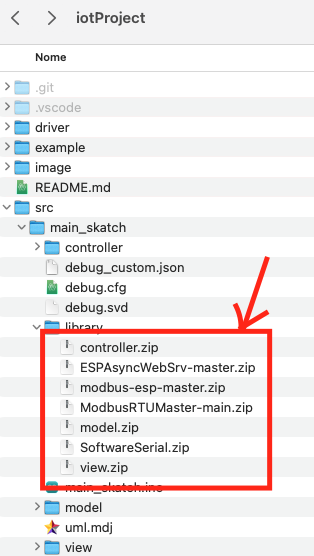
\includegraphics[width=0.3\linewidth]{../image/Library.png}
  \caption{Importazione delle librerie nell'Arduino IDE}
\end{figure}

\paragraph{} Altrimenti clonare la versione Portable del progetto disponibile al seguente link: \href{https://github.com/AlessioTommasi-supsi/iotProject/tree/portable}{iotProject-portable}.


\chapter{Hardware}
\section{Board Esam}
\subsection{Funzionamento}
\subsubsection{Multiplex}
\paragraph{ }
Il dispositivo di multiplexing riulta essere il \textbf{CD405xB}. \\
sviluppato da Texas Insreumet, link alla documentazione ufficiale: \href{https://www.ti.com/lit/ds/symlink/cd4051b.pdf}{CD405xB}. \\ 

Siccome successivamente servira diporto di seguito la tabella di verita di tale dispositivo. Figura 5.1 \\
\begin{figure}[H]
    \centering
    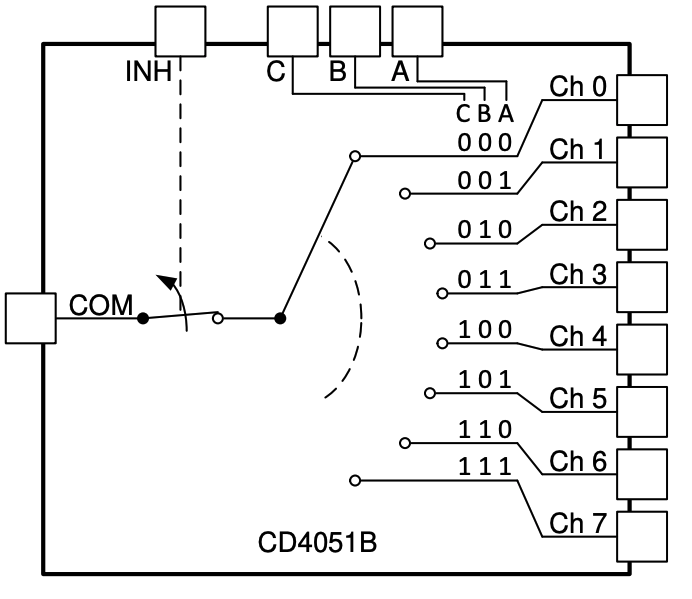
\includegraphics[width=0.5\linewidth]{../image/CD405xB.png}
    \caption{Tabella di verita del CD405xB}
\end{figure}

\subsubsection{Collegamenti Multiplexer}

I pin di ingresso A, B, C del multiplexer \textbf{CD405xB} sono collegati rispettivamente ai pin GPIO 12, 13, 14 dell'ESP32. La selezione dei canali del multiplexer avviene impostando i pin A, B, C come segue:

\begin{table}[H]
    \centering
    \begin{tabular}{|c|c|c|c|}
        \hline
        \textbf{Canale} & \textbf{Pin A} & \textbf{Pin B} & \textbf{Pin C} \\ \hline
        0 & 0 & 0 & 0 \\ \hline
        1 & 1 & 0 & 0 \\ \hline
        2 & 0 & 1 & 0 \\ \hline
        3 & 1 & 1 & 0 \\ \hline
        4 & 0 & 0 & 1 \\ \hline
        5 & 1 & 0 & 1 \\ \hline
        6 & 0 & 1 & 1 \\ \hline
        7 & 1 & 1 & 1 \\ \hline
    \end{tabular}
    \caption{Configurazione dei pin per la selezione dei canali del multiplexer}
\end{table}

\subsubsection{Canali Multiplexer}
Nella figura nella pagina seguente seguito vennogno riportati i collegamenti dei canali del multiplexer con i collegamenti esterni. 

\begin{figure}[H]
    \centering
    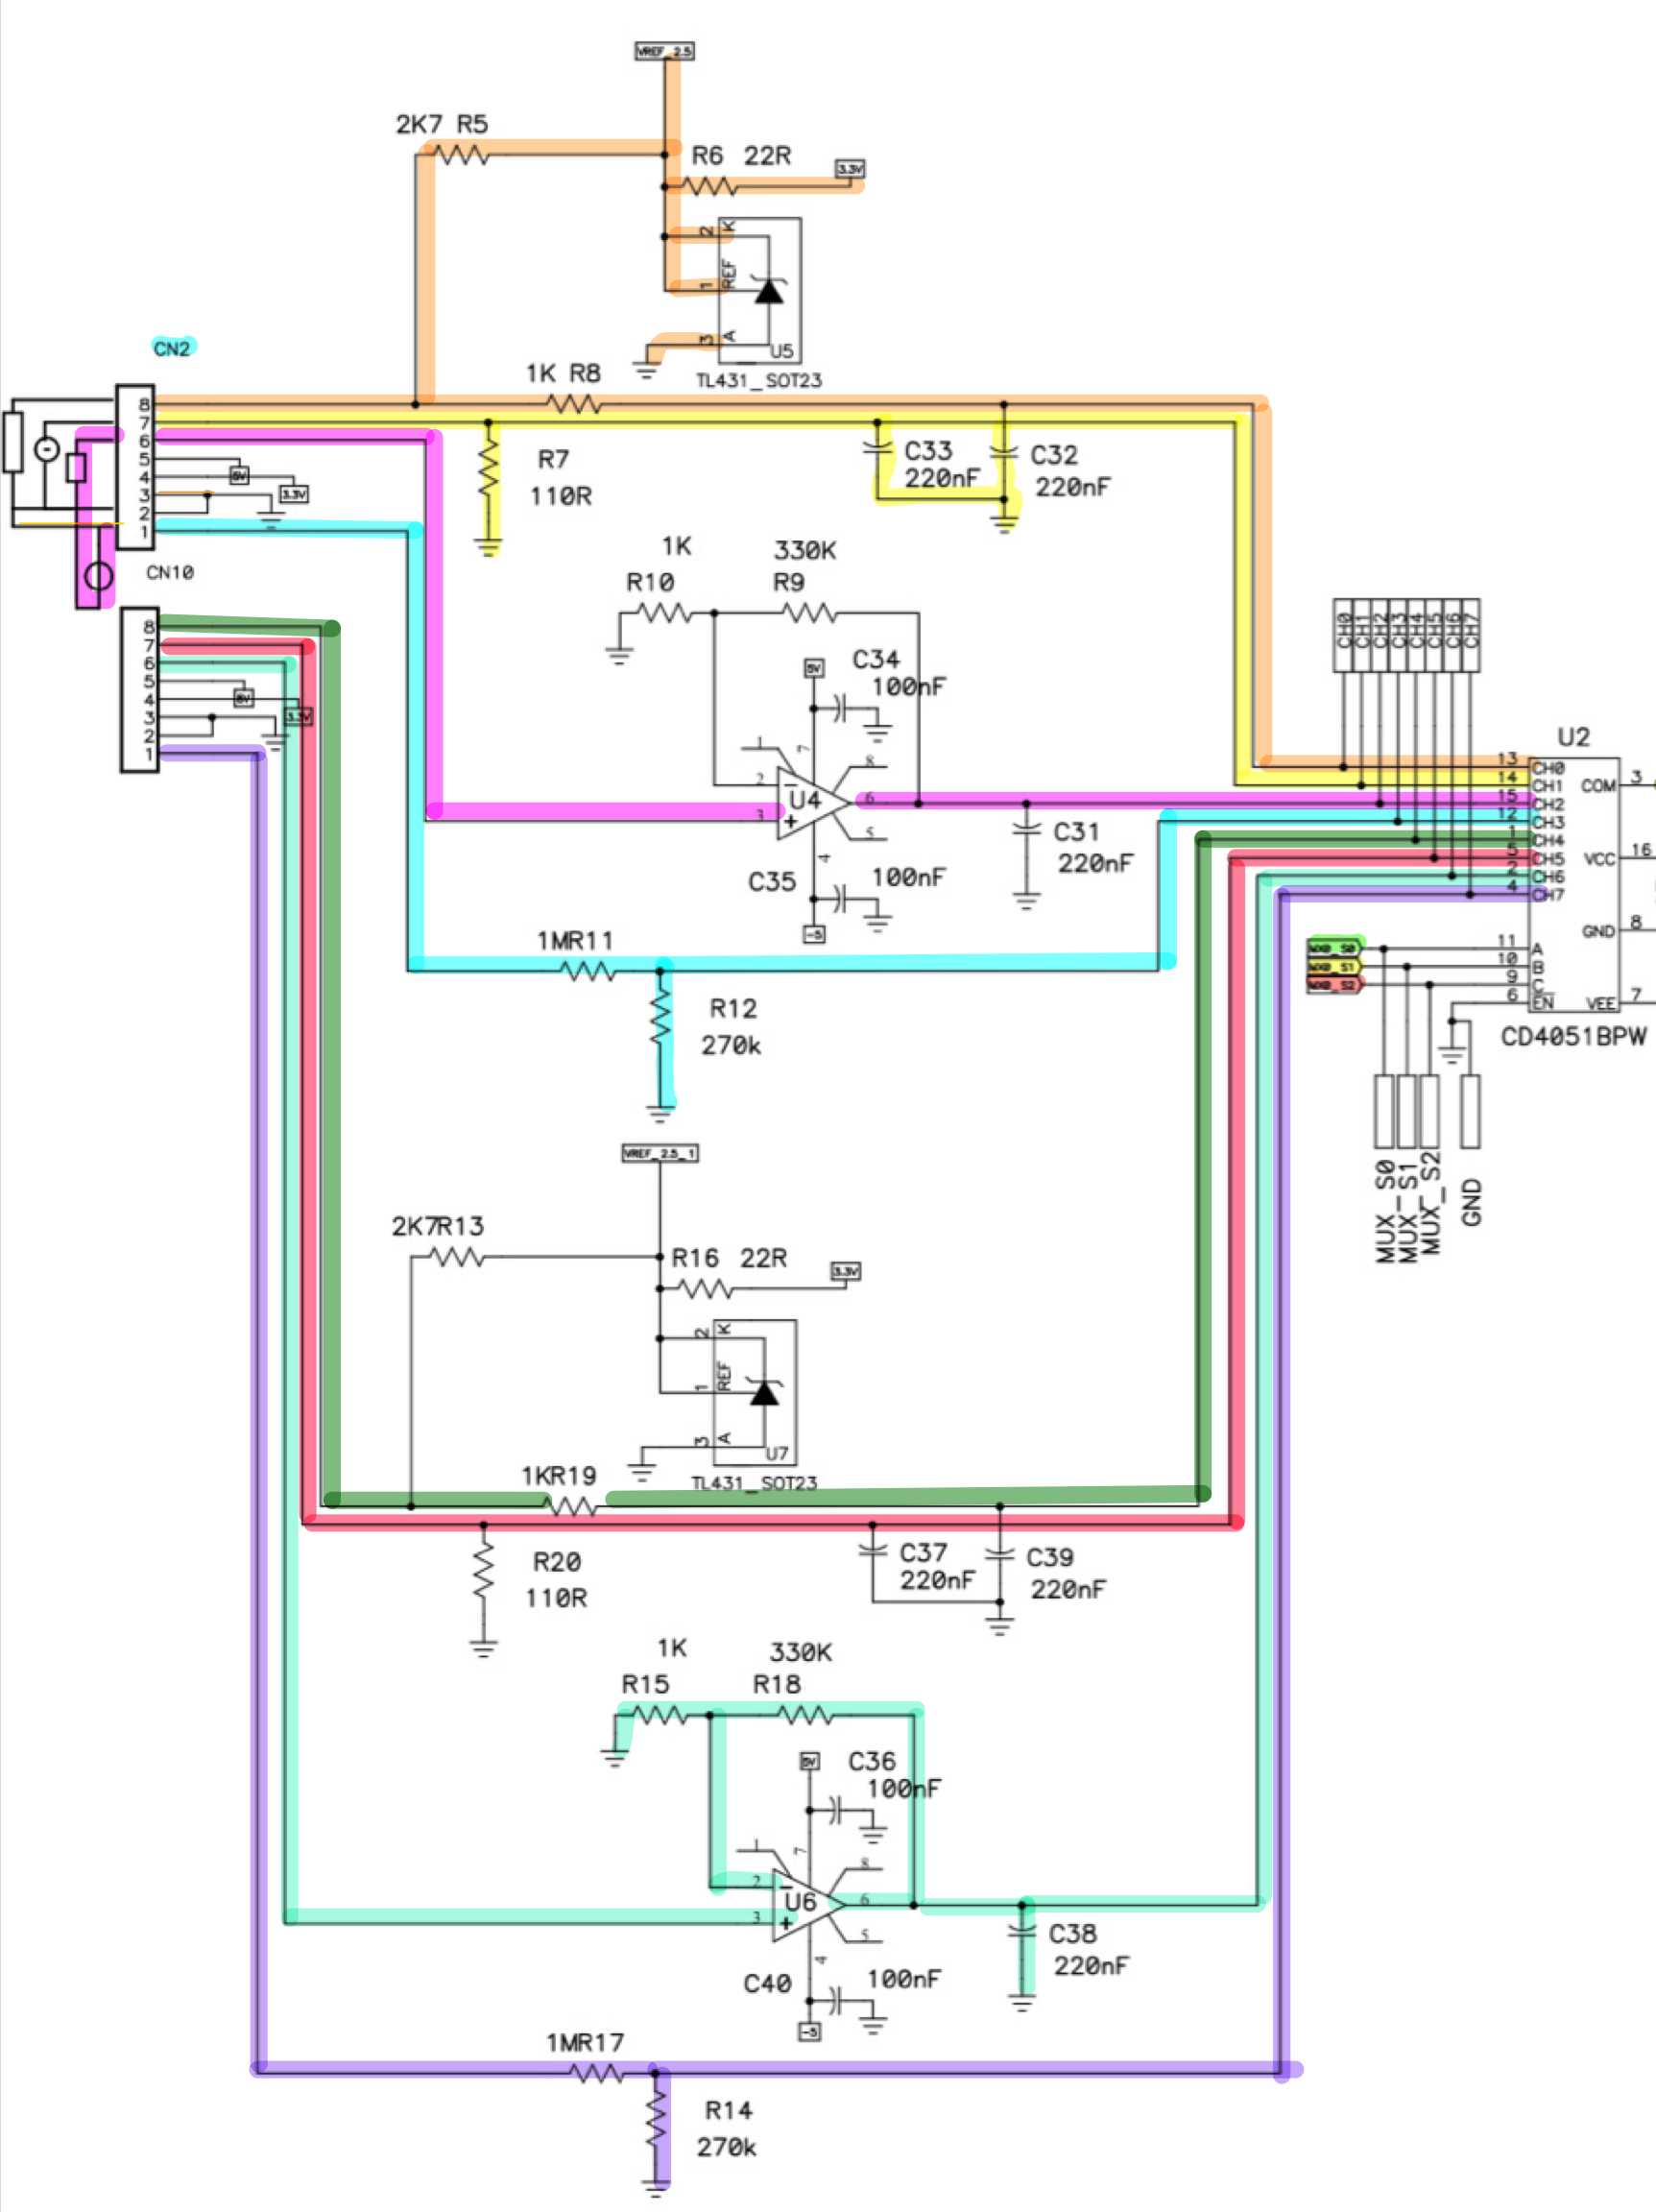
\includegraphics[width=\linewidth]{../image/channelMultiplex.png}
    \caption{Collegamenti dei canali del multiplexer}
\end{figure}

\paragraph{Ch0}
Selezionando Ch0 dall apposita pagina dedicata segue il percorso evidenziato in arancione nella Figura 5.2.
E' collegato a pin 8 della morsettiera CN2.
Su tale morsetto ci aspettiamo in ingresso un segnale di corrente che il componente TL431 si occupera di regolare e stabilizzare la tensione in ingresso entro dei range indicati.
a questo link potete trovare il datasheet di tale componente per maggiori info \href{https://www.ti.com/lit/ds/symlink/tl431.pdf}{TL431}.

\paragraph{Ch1}
percorso evidenziato in giallo nella Figura 5.2.

Possibili funzioni del segnale sul segnale in ingreso al pin 7 della morsettiera CN2.

- \textbf{Filtro Passa Basso}
Se il segnale applicato su R7 è una tensione alternata (AC), il circuito potrebbe attenuare le alte frequenze, lasciando passare solo le frequenze più basse

- \textbf{Stabilizzazione del segnale}

\paragraph{Ch2}
percorso evidenziato in viola nella Figura 5.2.

Leggeremo il segnale in ingresso al pin 6 della morsettiera CN2.

Il segnale verra amplificato dall operazionale U4 che e collegato come amplificatore non invertente (maggiori info al link \href{https://elettronicasemplice.weebly.com/amplificatore-operazionale-non-invertente.html}{LM358}).

Il guadagno di U4 e' dato dalla formula $G = 1 + \frac{R9}{R10}= 1+330 = 331 $.

inoltre tali alimentatore e alimentato tra 0 e +5v quindi clampera il segnale in ingresso tra 0 e +5v.
Il condensatore C31 si occupa di stabilizzare il segnale in uscita.

\paragraph{Ch3}
percorso evidenziato in azzurro nella Figura 5.2.

Leggeremo il segnale in ingresso al pin 1 della morsettiera CN2.

tra il segnale sul pin 1 ed ESP e'presente un partitore di tensione composto da R11 = 1M e R12 = 270K dunque $Vesp = Vpin1 * \frac{R12}{R11+R12} = Vpin1 * \frac{270}{1270} = Vpin1 * 0.2126$.


\paragraph{Ch4}
Connessione equivalente a CH0 

\paragraph{Ch5}
Connessione equivalente a CH1

\paragraph{Ch6}
Connessione equivalente a CH3

Tutte le connessioni equivalenti hanno un circuito hw separato per garantire la massima indipendenza tra i canali.
\subsection{ hardware esterno posizionabile sulla board}
\subsubsection{MAX31865}
asd

\subsubsection{ESP32 38 Pin}

\begin{figure}[H]
    \centering
    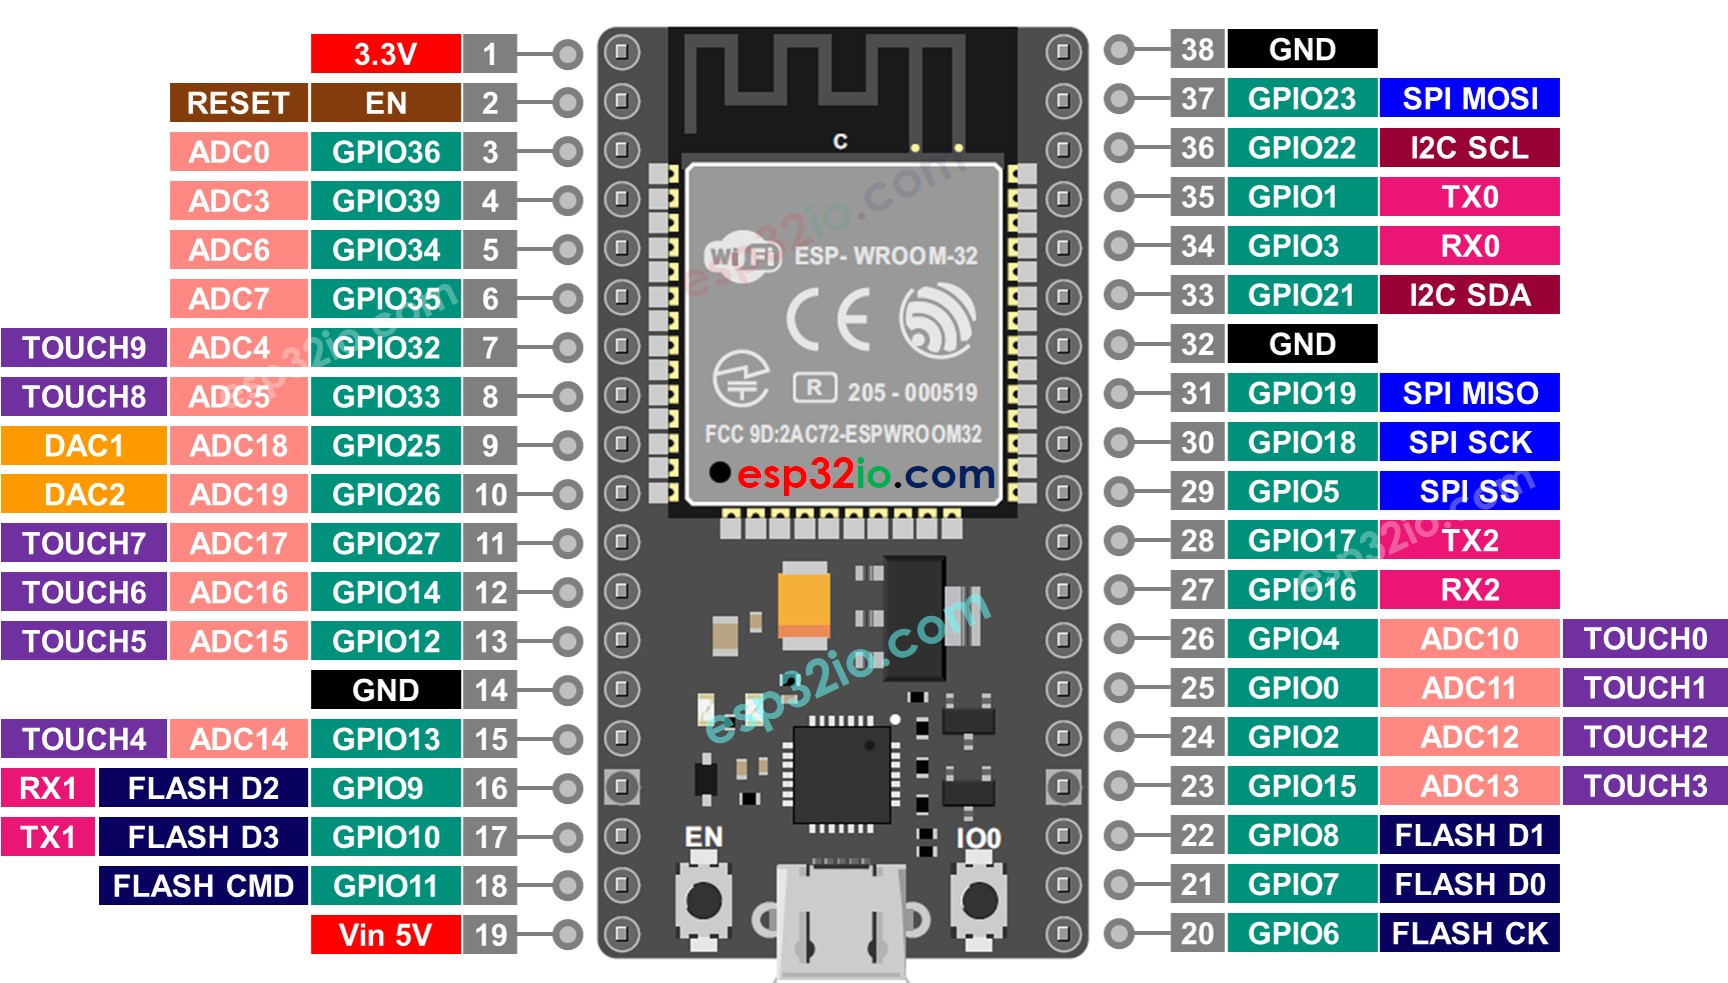
\includegraphics[width=\linewidth]{../image/ESP-38Pin-pinout.jpg}
    \caption{Pinout dell'ESP32-DOIT-DEV-KIT v1}
\end{figure}

\chapter{Software}
\section{Diagramma UML}
\begin{figure}[H]
    \centering
    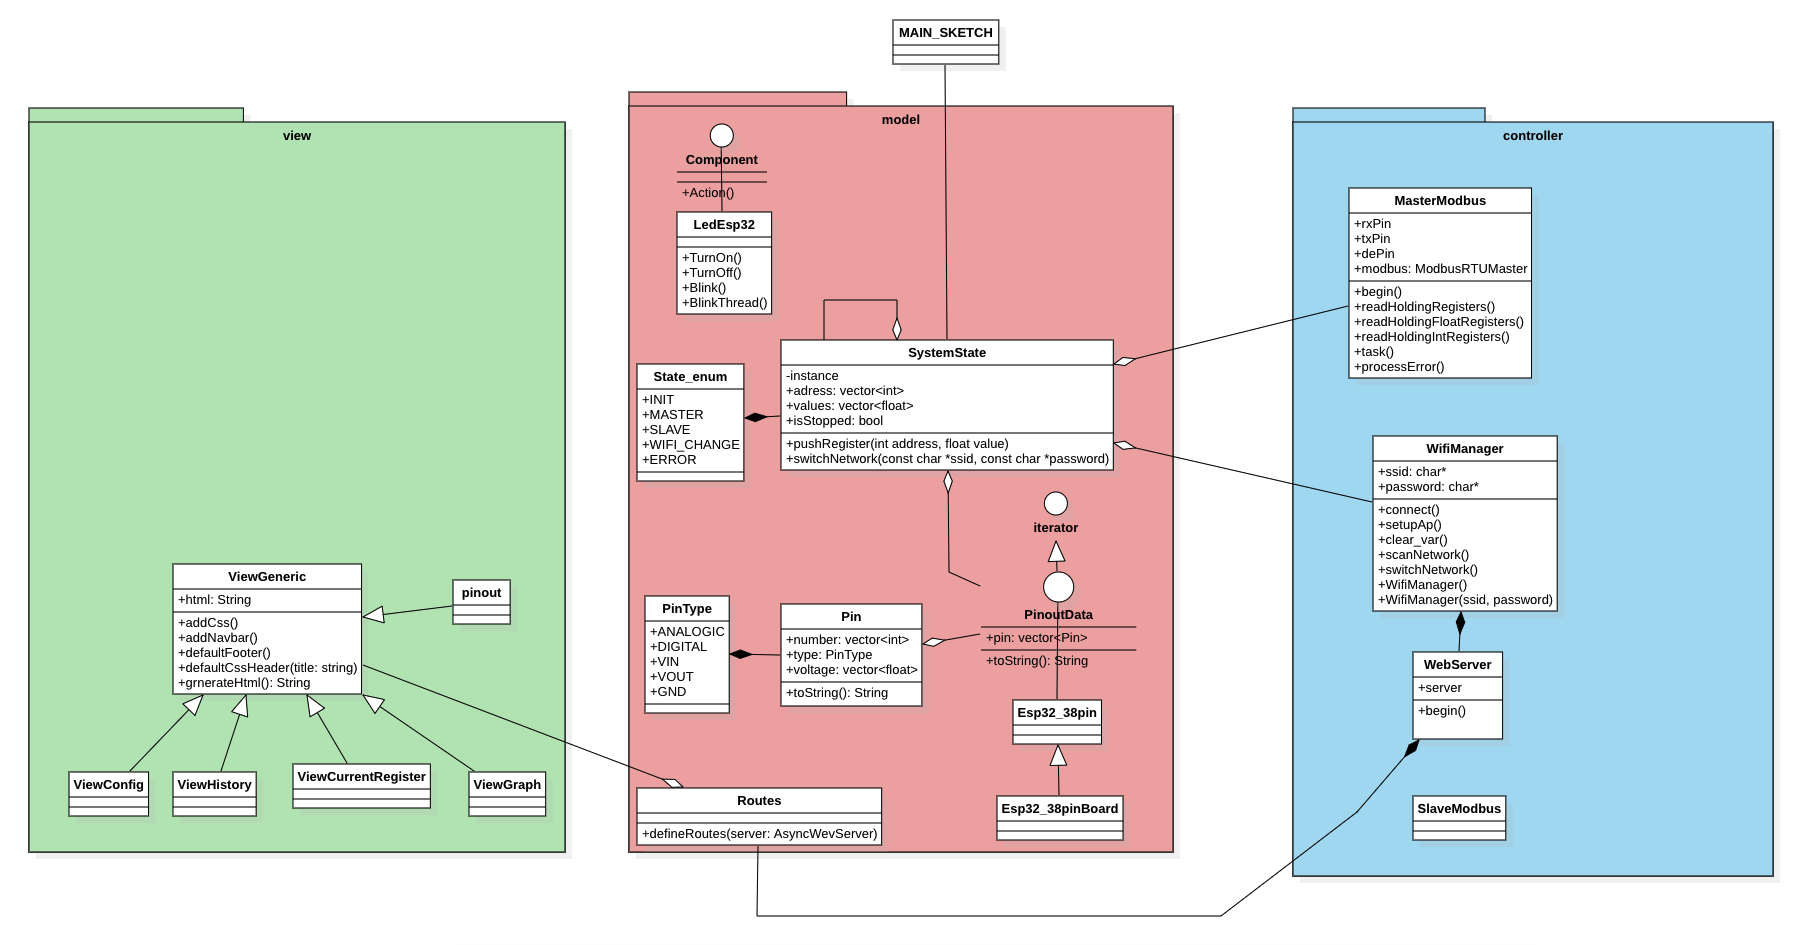
\includegraphics[width=\linewidth]{../image/uml.png}
    \caption{Diagramma UML del sistema}
\end{figure}
\subsection{Pattern}
\subsubsection{Model-View-Controller (MVC)}
\paragraph{Model} Contiene la struttura dei dati e le funzioni per accedere e modificarli. 
Le classi coinvolte sono \texttt{SystemState}, \texttt{Pin}, \texttt{PinoutData}, \texttt{Routes}.
\paragraph{View} Si occupa di visualizzare i dati e di interagire con l'utente.

principalmente sono classi che si occupano della generazione dei componenti delle pagine web visualizzate dall utente.

\paragraph{Controller} Gestisce le richieste dell'utente e aggiorna il modello di conseguenza.

\subsubsection{Singleton}
utilizzato per garantire unicita e atomicita dei dati \texttt{SystemState} e'la classe che implementa tale pattern.
Sara particolarmente utile in futuro per l'implementazione di un sistema di datalogging e persistenza dei dati su scheda SD.
\section{performace}
\section{WebServer}
\section{Modbus}
Il file utilizzato per testare lo slave è disponibile qui: \href{src/SLAVE\_EXAMPLE/modbusSlave2/modbusSlave2.ino}{modbusSlave2.ino}.

\begin{figure}[H]
    \centering
    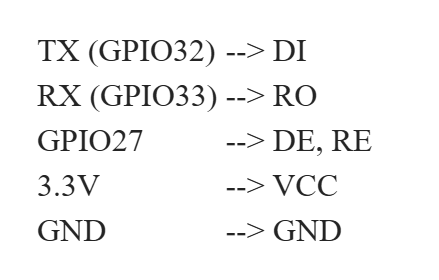
\includegraphics[width=\linewidth]{../image/SlavePinout.png}
    \caption{Pinout proposto per il dispositivo slave Modbus}
\end{figure}

\chapter{Attività}

\begin{longtable}{|p{0.35\textwidth}|p{0.65\textwidth}|}
\hline
\textbf{Attività} & \textbf{Descrizione} \\ \hline
\endfirsthead
\hline
\textbf{Attività} & \textbf{Descrizione} \\ \hline
\endhead
\hline
\endfoot
\textbf{Configurazione sensori di temperatura} & Configurare e integrare sensori di temperatura \textbf{PT100}, \textbf{PT1000} e \textbf{termocoppie} utilizzando moduli come \textbf{MAX31865} e \textbf{MAX31855}. \\ \hline
\textbf{Lettura segnali analogici} & Implementare la lettura di segnali analogici tramite gli ingressi \textbf{ADC} dell'ESP32 e eventuali moduli esterni. \\ \hline
\textbf{Gestione uscite digitali e analogiche} & Sviluppare la gestione delle uscite digitali e analogiche tramite l'ESP32. \\ \hline
\textbf{Comunicazione RS485 (Modbus RTU)} & Integrare la comunicazione \textbf{RS485} utilizzando il protocollo \textbf{Modbus RTU} per interfacciarsi con altri dispositivi. \\ \hline
\textbf{Server Web (Ethernet TCP/IP)} & Sviluppare un server \textbf{Web} basato su \textbf{Ethernet TCP/IP} per il monitoraggio e controllo remoto dei dati acquisiti. \\ \hline
\textbf{Datalogging} & Implementare un sistema di \textbf{datalogging} per salvare e storicizzare i dati raccolti dai sensori. \\ \hline
\textbf{Test e validazione} & Testare e validare il sistema attraverso simulazioni e test su hardware reale. \\ \hline
\end{longtable}

\chapter{Conclusioni}
\section{Sviluppi futuri}
\paragraph{persistenza e datalogging su scheda SD}
\paragraph{backup dati su cloud} implementazione backend etc
\section{Ringraziamenti}


\end{document}
